\documentclass[1p]{elsarticle_modified}
%\bibliographystyle{elsarticle-num}

%\usepackage[colorlinks]{hyperref}
%\usepackage{abbrmath_seonhwa} %\Abb, \Ascr, \Acal ,\Abf, \Afrak
\usepackage{amsfonts}
\usepackage{amssymb}
\usepackage{amsmath}
\usepackage{amsthm}
\usepackage{scalefnt}
\usepackage{amsbsy}
\usepackage{kotex}
\usepackage{caption}
\usepackage{subfig}
\usepackage{color}
\usepackage{graphicx}
\usepackage{xcolor} %% white, black, red, green, blue, cyan, magenta, yellow
\usepackage{float}
\usepackage{setspace}
\usepackage{hyperref}

\usepackage{tikz}
\usetikzlibrary{arrows}

\usepackage{multirow}
\usepackage{array} % fixed length table
\usepackage{hhline}

%%%%%%%%%%%%%%%%%%%%%
\makeatletter
\renewcommand*\env@matrix[1][\arraystretch]{%
	\edef\arraystretch{#1}%
	\hskip -\arraycolsep
	\let\@ifnextchar\new@ifnextchar
	\array{*\c@MaxMatrixCols c}}
\makeatother %https://tex.stackexchange.com/questions/14071/how-can-i-increase-the-line-spacing-in-a-matrix
%%%%%%%%%%%%%%%

\usepackage[normalem]{ulem}

\newcommand{\msout}[1]{\ifmmode\text{\sout{\ensuremath{#1}}}\else\sout{#1}\fi}
%SOURCE: \msout is \stkout macro in https://tex.stackexchange.com/questions/20609/strikeout-in-math-mode

\newcommand{\cancel}[1]{
	\ifmmode
	{\color{red}\msout{#1}}
	\else
	{\color{red}\sout{#1}}
	\fi
}

\newcommand{\add}[1]{
	{\color{blue}\uwave{#1}}
}

\newcommand{\replace}[2]{
	\ifmmode
	{\color{red}\msout{#1}}{\color{blue}\uwave{#2}}
	\else
	{\color{red}\sout{#1}}{\color{blue}\uwave{#2}}
	\fi
}

\newcommand{\Sol}{\mathcal{S}} %segment
\newcommand{\D}{D} %diagram
\newcommand{\A}{\mathcal{A}} %arc


%%%%%%%%%%%%%%%%%%%%%%%%%%%%%5 test

\def\sl{\operatorname{\textup{SL}}(2,\Cbb)}
\def\psl{\operatorname{\textup{PSL}}(2,\Cbb)}
\def\quan{\mkern 1mu \triangleright \mkern 1mu}

\theoremstyle{definition}
\newtheorem{thm}{Theorem}[section]
\newtheorem{prop}[thm]{Proposition}
\newtheorem{lem}[thm]{Lemma}
\newtheorem{ques}[thm]{Question}
\newtheorem{cor}[thm]{Corollary}
\newtheorem{defn}[thm]{Definition}
\newtheorem{exam}[thm]{Example}
\newtheorem{rmk}[thm]{Remark}
\newtheorem{alg}[thm]{Algorithm}

\newcommand{\I}{\sqrt{-1}}
\begin{document}

%\begin{frontmatter}
%
%\title{Boundary parabolic representations of knots up to 8 crossings}
%
%%% Group authors per affiliation:
%\author{Yunhi Cho} 
%\address{Department of Mathematics, University of Seoul, Seoul, Korea}
%\ead{yhcho@uos.ac.kr}
%
%
%\author{Seonhwa Kim} %\fnref{s_kim}}
%\address{Center for Geometry and Physics, Institute for Basic Science, Pohang, 37673, Korea}
%\ead{ryeona17@ibs.re.kr}
%
%\author{Hyuk Kim}
%\address{Department of Mathematical Sciences, Seoul National University, Seoul 08826, Korea}
%\ead{hyukkim@snu.ac.kr}
%
%\author{Seokbeom Yoon}
%\address{Department of Mathematical Sciences, Seoul National University, Seoul, 08826,  Korea}
%\ead{sbyoon15@snu.ac.kr}
%
%\begin{abstract}
%We find all boundary parabolic representation of knots up to 8 crossings.
%
%\end{abstract}
%\begin{keyword}
%    \MSC[2010] 57M25 
%\end{keyword}
%
%\end{frontmatter}

%\linenumbers
%\tableofcontents
%
\newcommand\colored[1]{\textcolor{white}{\rule[-0.35ex]{0.8em}{1.4ex}}\kern-0.8em\color{red} #1}%
%\newcommand\colored[1]{\textcolor{white}{ #1}\kern-2.17ex	\textcolor{white}{ #1}\kern-1.81ex	\textcolor{white}{ #1}\kern-2.15ex\color{red}#1	}

{\Large $\underline{11a_{286}~(K11a_{286})}$}

\setlength{\tabcolsep}{10pt}
\renewcommand{\arraystretch}{1.6}
\vspace{1cm}\begin{tabular}{m{100pt}>{\centering\arraybackslash}m{274pt}}
\multirow{5}{120pt}{
	\centering
	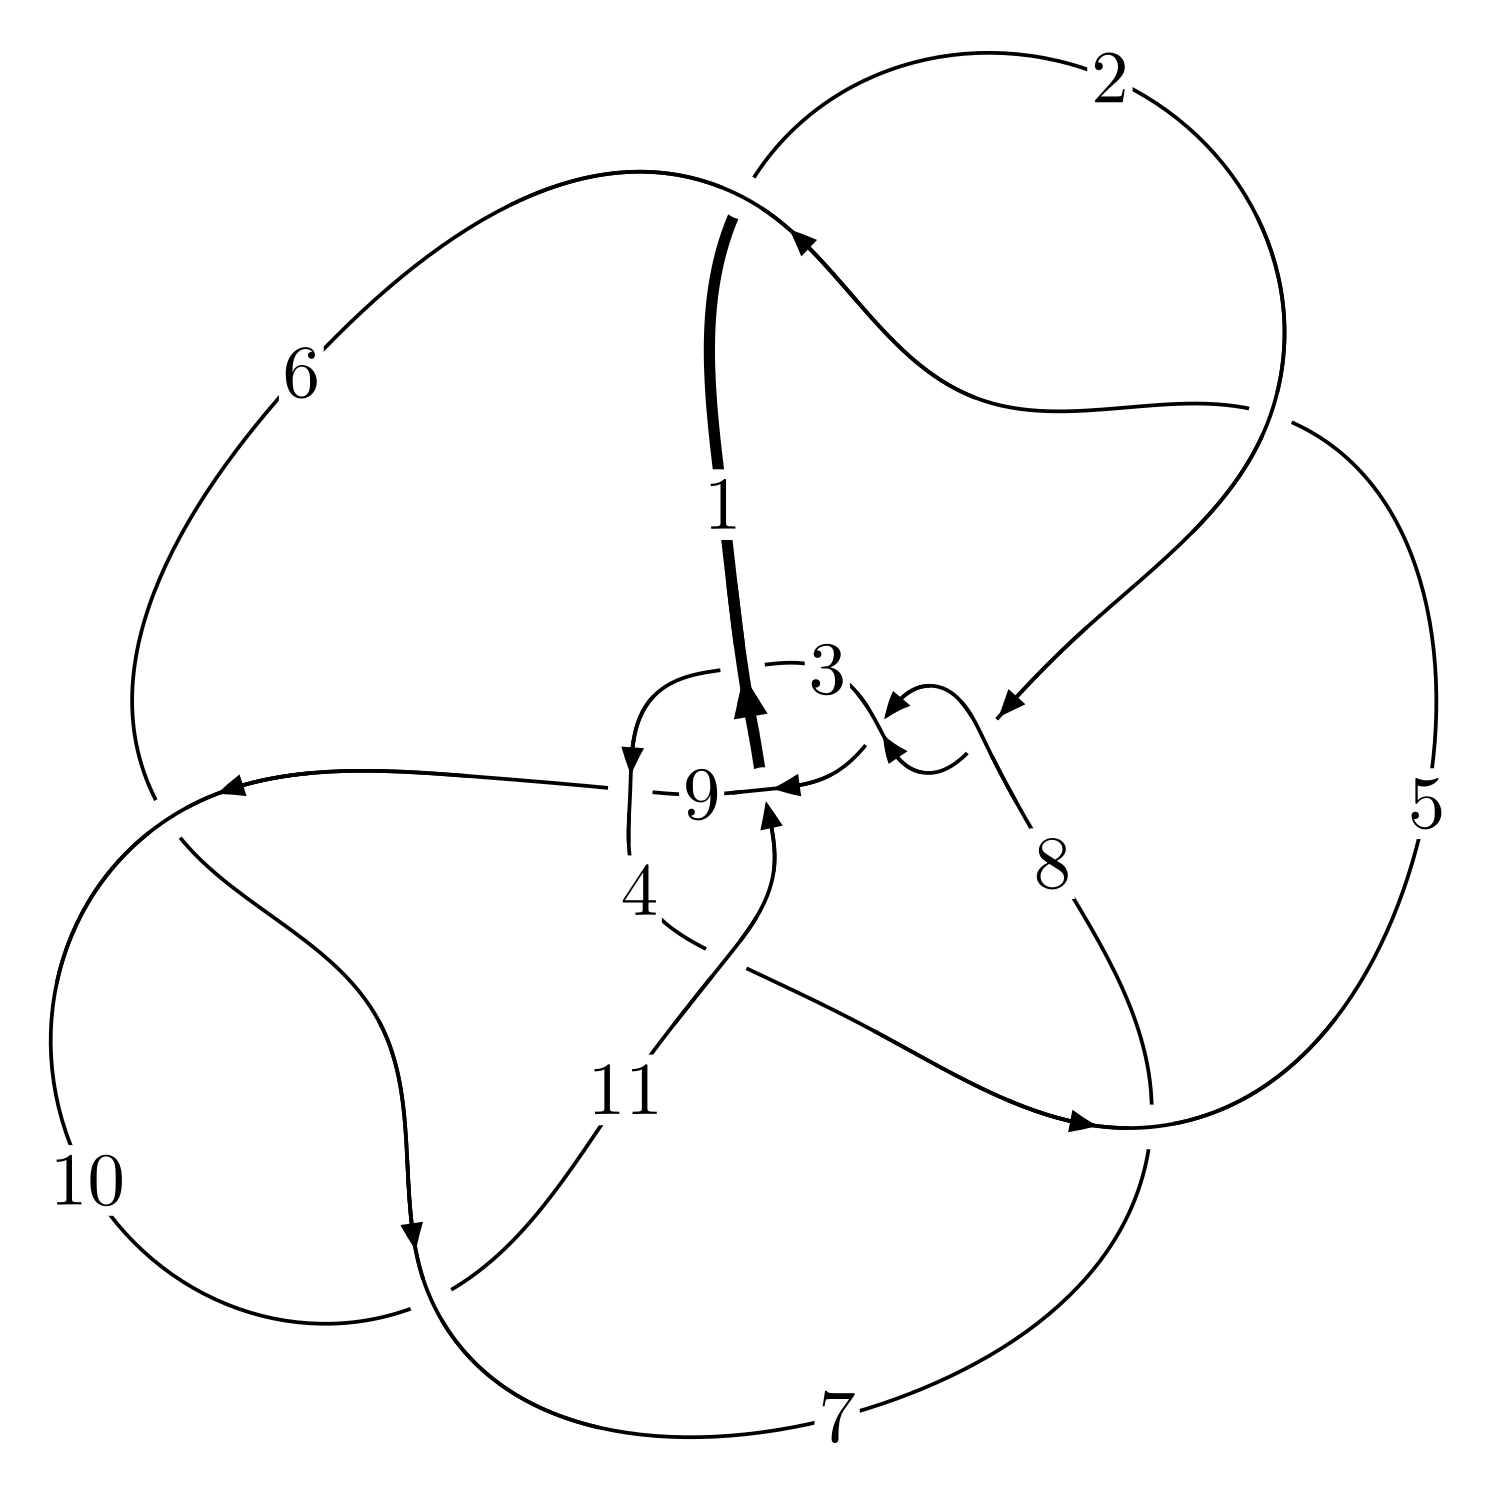
\includegraphics[width=112pt]{../../../GIT/diagram.site/Diagrams/png/535_11a_286.png}\\
\ \ \ A knot diagram\footnotemark}&
\allowdisplaybreaks
\textbf{Linearized knot diagam} \\
\cline{2-2}
 &
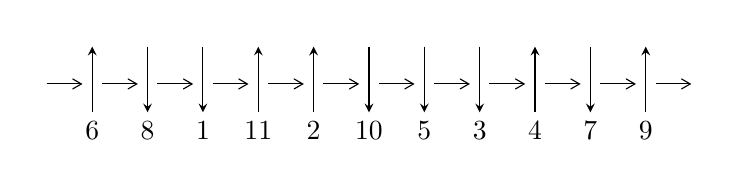
\begin{tikzpicture}[x=20pt, y=17pt]
	% nodes
	\node (C0) at (0, 0) {};
	\node (C1) at (1, 0) {};
	\node (C1U) at (1, +1) {};
	\node (C1D) at (1, -1) {6};

	\node (C2) at (2, 0) {};
	\node (C2U) at (2, +1) {};
	\node (C2D) at (2, -1) {8};

	\node (C3) at (3, 0) {};
	\node (C3U) at (3, +1) {};
	\node (C3D) at (3, -1) {1};

	\node (C4) at (4, 0) {};
	\node (C4U) at (4, +1) {};
	\node (C4D) at (4, -1) {11};

	\node (C5) at (5, 0) {};
	\node (C5U) at (5, +1) {};
	\node (C5D) at (5, -1) {2};

	\node (C6) at (6, 0) {};
	\node (C6U) at (6, +1) {};
	\node (C6D) at (6, -1) {10};

	\node (C7) at (7, 0) {};
	\node (C7U) at (7, +1) {};
	\node (C7D) at (7, -1) {5};

	\node (C8) at (8, 0) {};
	\node (C8U) at (8, +1) {};
	\node (C8D) at (8, -1) {3};

	\node (C9) at (9, 0) {};
	\node (C9U) at (9, +1) {};
	\node (C9D) at (9, -1) {4};

	\node (C10) at (10, 0) {};
	\node (C10U) at (10, +1) {};
	\node (C10D) at (10, -1) {7};

	\node (C11) at (11, 0) {};
	\node (C11U) at (11, +1) {};
	\node (C11D) at (11, -1) {9};
	\node (C12) at (12, 0) {};

	% arrows
	\draw[->,>={angle 60}]
	(C0) edge (C1) (C1) edge (C2) (C2) edge (C3) (C3) edge (C4) (C4) edge (C5) (C5) edge (C6) (C6) edge (C7) (C7) edge (C8) (C8) edge (C9) (C9) edge (C10) (C10) edge (C11) (C11) edge (C12) ;	\draw[->,>=stealth]
	(C1D) edge (C1U) (C2U) edge (C2D) (C3U) edge (C3D) (C4D) edge (C4U) (C5D) edge (C5U) (C6U) edge (C6D) (C7U) edge (C7D) (C8U) edge (C8D) (C9D) edge (C9U) (C10U) edge (C10D) (C11D) edge (C11U) ;
	\end{tikzpicture} \\
\hhline{~~} \\& 
\textbf{Solving Sequence} \\ \cline{2-2} 
 &
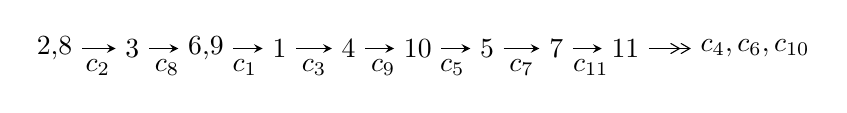
\begin{tikzpicture}[x=25pt, y=7pt]
	% node
	\node (A0) at (-1/8, 0) {2,8};
	\node (A1) at (1, 0) {3};
	\node (A2) at (33/16, 0) {6,9};
	\node (A3) at (25/8, 0) {1};
	\node (A4) at (33/8, 0) {4};
	\node (A5) at (41/8, 0) {10};
	\node (A6) at (49/8, 0) {5};
	\node (A7) at (57/8, 0) {7};
	\node (A8) at (65/8, 0) {11};
	\node (C1) at (1/2, -1) {$c_{2}$};
	\node (C2) at (3/2, -1) {$c_{8}$};
	\node (C3) at (21/8, -1) {$c_{1}$};
	\node (C4) at (29/8, -1) {$c_{3}$};
	\node (C5) at (37/8, -1) {$c_{9}$};
	\node (C6) at (45/8, -1) {$c_{5}$};
	\node (C7) at (53/8, -1) {$c_{7}$};
	\node (C8) at (61/8, -1) {$c_{11}$};
	\node (A9) at (10, 0) {$c_{4},c_{6},c_{10}$};

	% edge
	\draw[->,>=stealth]	
	(A0) edge (A1) (A1) edge (A2) (A2) edge (A3) (A3) edge (A4) (A4) edge (A5) (A5) edge (A6) (A6) edge (A7) (A7) edge (A8) ;
	\draw[->>,>={angle 60}]	
	(A8) edge (A9);
\end{tikzpicture} \\ 

\end{tabular} \\

\footnotetext{
The image of knot diagram is generated by the software ``\textbf{Draw programme}" developed by Andrew Bartholomew(\url{http://www.layer8.co.uk/maths/draw/index.htm\#Running-draw}), where we modified some parts for our purpose(\url{https://github.com/CATsTAILs/LinksPainter}).
}\phantom \\ \newline 
\centering \textbf{Ideals for irreducible components\footnotemark of $X_{\text{par}}$} 
 
\begin{align*}
I^u_{1}&=\langle 
-1.55234\times10^{267} u^{88}-4.31282\times10^{267} u^{87}+\cdots+1.32472\times10^{270} b-3.32772\times10^{270},\\
\phantom{I^u_{1}}&\phantom{= \langle  }-9.22601\times10^{271} u^{88}+1.62321\times10^{271} u^{87}+\cdots+5.74253\times10^{274} a-3.46330\times10^{275},\\
\phantom{I^u_{1}}&\phantom{= \langle  }u^{89}+2 u^{88}+\cdots-1333 u+647\rangle \\
I^u_{2}&=\langle 
-5635742 u^{22}+8544802 u^{21}+\cdots+1559171 b-7785518,\\
\phantom{I^u_{2}}&\phantom{= \langle  }-175768102 u^{22}+289559314 u^{21}+\cdots+45215959 a-268721385,\;u^{23}- u^{22}+\cdots+3 u+1\rangle \\
I^u_{3}&=\langle 
- u^2+b,\;a-1,\;u^6+u^5-1\rangle \\
I^u_{4}&=\langle 
b-1,\;a-1,\;u-1\rangle \\
\\
\end{align*}
\raggedright * 4 irreducible components of $\dim_{\mathbb{C}}=0$, with total 119 representations.\\
\footnotetext{All coefficients of polynomials are rational numbers. But the coefficients are sometimes approximated in decimal forms when there is not enough margin.}
\newpage
\renewcommand{\arraystretch}{1}
\centering \section*{I. $I^u_{1}= \langle -1.55\times10^{267} u^{88}-4.31\times10^{267} u^{87}+\cdots+1.32\times10^{270} b-3.33\times10^{270},\;-9.23\times10^{271} u^{88}+1.62\times10^{271} u^{87}+\cdots+5.74\times10^{274} a-3.46\times10^{275},\;u^{89}+2 u^{88}+\cdots-1333 u+647 \rangle$}
\flushleft \textbf{(i) Arc colorings}\\
\begin{tabular}{m{7pt} m{180pt} m{7pt} m{180pt} }
\flushright $a_{2}=$&$\begin{pmatrix}1\\0\end{pmatrix}$ \\
\flushright $a_{8}=$&$\begin{pmatrix}0\\u\end{pmatrix}$ \\
\flushright $a_{3}=$&$\begin{pmatrix}1\\u^2\end{pmatrix}$ \\
\flushright $a_{6}=$&$\begin{pmatrix}0.00160661 u^{88}-0.000282665 u^{87}+\cdots-11.9326 u+6.03096\\0.00117182 u^{88}+0.00325564 u^{87}+\cdots+3.24187 u+2.51202\end{pmatrix}$ \\
\flushright $a_{9}=$&$\begin{pmatrix}- u\\- u^3+u\end{pmatrix}$ \\
\flushright $a_{1}=$&$\begin{pmatrix}0.00318081 u^{88}+0.00410332 u^{87}+\cdots+3.56991 u+5.20178\\0.00290796 u^{88}+0.00391365 u^{87}+\cdots-7.38301 u+2.72421\end{pmatrix}$ \\
\flushright $a_{4}=$&$\begin{pmatrix}-0.00181149 u^{88}-0.00607733 u^{87}+\cdots-12.3004 u+7.55856\\0.00916924 u^{88}+0.0106604 u^{87}+\cdots-4.14988 u+0.678788\end{pmatrix}$ \\
\flushright $a_{10}=$&$\begin{pmatrix}0.00119620 u^{88}-0.00157570 u^{87}+\cdots-8.00639 u-3.80599\\-0.00146737 u^{88}+0.00122998 u^{87}+\cdots+10.8586 u-0.0804670\end{pmatrix}$ \\
\flushright $a_{5}=$&$\begin{pmatrix}0.000434788 u^{88}-0.00353831 u^{87}+\cdots-15.1744 u+3.51894\\0.00117182 u^{88}+0.00325564 u^{87}+\cdots+3.24187 u+2.51202\end{pmatrix}$ \\
\flushright $a_{7}=$&$\begin{pmatrix}0.00590099 u^{88}-0.00142517 u^{87}+\cdots-16.2111 u+13.2628\\-0.000356025 u^{88}-0.000216007 u^{87}+\cdots+2.84127 u-0.176532\end{pmatrix}$ \\
\flushright $a_{11}=$&$\begin{pmatrix}0.00351260 u^{88}+0.00181198 u^{87}+\cdots+1.84399 u+5.88592\\0.00567299 u^{88}+0.00695895 u^{87}+\cdots-9.81067 u+3.95191\end{pmatrix}$\\ \flushright $a_{11}=$&$\begin{pmatrix}0.00351260 u^{88}+0.00181198 u^{87}+\cdots+1.84399 u+5.88592\\0.00567299 u^{88}+0.00695895 u^{87}+\cdots-9.81067 u+3.95191\end{pmatrix}$\\&\end{tabular}
\flushleft \textbf{(ii) Obstruction class $= -1$}\\~\\
\flushleft \textbf{(iii) Cusp Shapes $= 0.0524832 u^{88}+0.137268 u^{87}+\cdots+11.5462 u-2.46166$}\\~\\
\newpage\renewcommand{\arraystretch}{1}
\flushleft \textbf{(iv) u-Polynomials at the component}\newline \\
\begin{tabular}{m{50pt}|m{274pt}}
Crossings & \hspace{64pt}u-Polynomials at each crossing \\
\hline $$\begin{aligned}c_{1},c_{5}\end{aligned}$$&$\begin{aligned}
&u^{89}-2 u^{88}+\cdots+90320 u+7513
\end{aligned}$\\
\hline $$\begin{aligned}c_{2},c_{8}\end{aligned}$$&$\begin{aligned}
&u^{89}-2 u^{88}+\cdots-1333 u-647
\end{aligned}$\\
\hline $$\begin{aligned}c_{3}\end{aligned}$$&$\begin{aligned}
&u^{89}-11 u^{88}+\cdots+527 u-23
\end{aligned}$\\
\hline $$\begin{aligned}c_{4}\end{aligned}$$&$\begin{aligned}
&u^{89}-5 u^{88}+\cdots+635519 u+52123
\end{aligned}$\\
\hline $$\begin{aligned}c_{6},c_{10}\end{aligned}$$&$\begin{aligned}
&u^{89}-5 u^{88}+\cdots-2896 u+424
\end{aligned}$\\
\hline $$\begin{aligned}c_{7}\end{aligned}$$&$\begin{aligned}
&u^{89}-6 u^{88}+\cdots+521820 u+24583
\end{aligned}$\\
\hline $$\begin{aligned}c_{9}\end{aligned}$$&$\begin{aligned}
&u^{89}+u^{88}+\cdots-19 u-1
\end{aligned}$\\
\hline $$\begin{aligned}c_{11}\end{aligned}$$&$\begin{aligned}
&u^{89}+14 u^{88}+\cdots-5718 u-557
\end{aligned}$\\
\hline
\end{tabular}\\~\\
\newpage\renewcommand{\arraystretch}{1}
\flushleft \textbf{(v) Riley Polynomials at the component}\newline \\
\begin{tabular}{m{50pt}|m{274pt}}
Crossings & \hspace{64pt}Riley Polynomials at each crossing \\
\hline $$\begin{aligned}c_{1},c_{5}\end{aligned}$$&$\begin{aligned}
&y^{89}+64 y^{88}+\cdots-300613312 y-56445169
\end{aligned}$\\
\hline $$\begin{aligned}c_{2},c_{8}\end{aligned}$$&$\begin{aligned}
&y^{89}-80 y^{88}+\cdots+3896461 y-418609
\end{aligned}$\\
\hline $$\begin{aligned}c_{3}\end{aligned}$$&$\begin{aligned}
&y^{89}-21 y^{88}+\cdots+57481 y-529
\end{aligned}$\\
\hline $$\begin{aligned}c_{4}\end{aligned}$$&$\begin{aligned}
&y^{89}+31 y^{88}+\cdots-29419728923 y-2716807129
\end{aligned}$\\
\hline $$\begin{aligned}c_{6},c_{10}\end{aligned}$$&$\begin{aligned}
&y^{89}-61 y^{88}+\cdots+3809312 y-179776
\end{aligned}$\\
\hline $$\begin{aligned}c_{7}\end{aligned}$$&$\begin{aligned}
&y^{89}-42 y^{88}+\cdots+387303203794 y-604323889
\end{aligned}$\\
\hline $$\begin{aligned}c_{9}\end{aligned}$$&$\begin{aligned}
&y^{89}+y^{88}+\cdots+201 y-1
\end{aligned}$\\
\hline $$\begin{aligned}c_{11}\end{aligned}$$&$\begin{aligned}
&y^{89}+6 y^{88}+\cdots-11245092 y-310249
\end{aligned}$\\
\hline
\end{tabular}\\~\\
\newpage\flushleft \textbf{(vi) Complex Volumes and Cusp Shapes}
$$\begin{array}{c|c|c}  
\text{Solutions to }I^u_{1}& \I (\text{vol} + \sqrt{-1}CS) & \text{Cusp shape}\\
 \hline 
\begin{aligned}
u &= -0.852038 + 0.573966 I \\
a &= \phantom{-}0.153177 + 0.809297 I \\
b &= \phantom{-}0.419729 + 0.323128 I\end{aligned}
 & \phantom{-}1.05660 + 4.06132 I & \phantom{-0.000000 } 0 \\ \hline\begin{aligned}
u &= -0.852038 - 0.573966 I \\
a &= \phantom{-}0.153177 - 0.809297 I \\
b &= \phantom{-}0.419729 - 0.323128 I\end{aligned}
 & \phantom{-}1.05660 - 4.06132 I & \phantom{-0.000000 } 0 \\ \hline\begin{aligned}
u &= -0.864849 + 0.385795 I \\
a &= \phantom{-}0.241214 + 0.307598 I \\
b &= -0.308549 - 0.832916 I\end{aligned}
 & -2.04087 + 4.73072 I & \phantom{-0.000000 } 0 \\ \hline\begin{aligned}
u &= -0.864849 - 0.385795 I \\
a &= \phantom{-}0.241214 - 0.307598 I \\
b &= -0.308549 + 0.832916 I\end{aligned}
 & -2.04087 - 4.73072 I & \phantom{-0.000000 } 0 \\ \hline\begin{aligned}
u &= \phantom{-}0.932246\phantom{ +0.000000I} \\
a &= \phantom{-}1.02505\phantom{ +0.000000I} \\
b &= \phantom{-}0.898656\phantom{ +0.000000I}\end{aligned}
 & -1.64367\phantom{ +0.000000I} & \phantom{-0.000000 } 0 \\ \hline\begin{aligned}
u &= -1.140430 + 0.113727 I \\
a &= \phantom{-}0.33690 - 2.20649 I \\
b &= \phantom{-}0.270332 - 1.071420 I\end{aligned}
 & -3.93177 - 3.22400 I & \phantom{-0.000000 } 0 \\ \hline\begin{aligned}
u &= -1.140430 - 0.113727 I \\
a &= \phantom{-}0.33690 + 2.20649 I \\
b &= \phantom{-}0.270332 + 1.071420 I\end{aligned}
 & -3.93177 + 3.22400 I & \phantom{-0.000000 } 0 \\ \hline\begin{aligned}
u &= \phantom{-}1.15466\phantom{ +0.000000I} \\
a &= -1.55856\phantom{ +0.000000I} \\
b &= -2.53211\phantom{ +0.000000I}\end{aligned}
 & -3.85286\phantom{ +0.000000I} & \phantom{-0.000000 } 0 \\ \hline\begin{aligned}
u &= -0.460947 + 0.694535 I \\
a &= \phantom{-}1.310850 + 0.249643 I \\
b &= -0.575229 + 0.865518 I\end{aligned}
 & -2.26703 - 4.51831 I & -7.03491 + 7.29654 I \\ \hline\begin{aligned}
u &= -0.460947 - 0.694535 I \\
a &= \phantom{-}1.310850 - 0.249643 I \\
b &= -0.575229 - 0.865518 I\end{aligned}
 & -2.26703 + 4.51831 I & -7.03491 - 7.29654 I\\
 \hline 
 \end{array}$$\newpage$$\begin{array}{c|c|c}  
\text{Solutions to }I^u_{1}& \I (\text{vol} + \sqrt{-1}CS) & \text{Cusp shape}\\
 \hline 
\begin{aligned}
u &= \phantom{-}1.182030 + 0.111716 I \\
a &= \phantom{-}0.026577 + 1.131400 I \\
b &= -1.10640 + 1.13771 I\end{aligned}
 & -4.32016 - 0.46135 I & \phantom{-0.000000 } 0 \\ \hline\begin{aligned}
u &= \phantom{-}1.182030 - 0.111716 I \\
a &= \phantom{-}0.026577 - 1.131400 I \\
b &= -1.10640 - 1.13771 I\end{aligned}
 & -4.32016 + 0.46135 I & \phantom{-0.000000 } 0 \\ \hline\begin{aligned}
u &= \phantom{-}1.052700 + 0.579893 I \\
a &= \phantom{-}0.240171 - 0.373271 I \\
b &= \phantom{-}0.470747 + 0.682507 I\end{aligned}
 & -3.68792 - 5.17721 I & \phantom{-0.000000 } 0 \\ \hline\begin{aligned}
u &= \phantom{-}1.052700 - 0.579893 I \\
a &= \phantom{-}0.240171 + 0.373271 I \\
b &= \phantom{-}0.470747 - 0.682507 I\end{aligned}
 & -3.68792 + 5.17721 I & \phantom{-0.000000 } 0 \\ \hline\begin{aligned}
u &= -0.071192 + 0.780803 I \\
a &= \phantom{-}0.333783 + 0.327684 I \\
b &= \phantom{-}0.391335 - 1.253760 I\end{aligned}
 & -4.73333 - 5.13676 I & -4.79385 + 5.15866 I \\ \hline\begin{aligned}
u &= -0.071192 - 0.780803 I \\
a &= \phantom{-}0.333783 - 0.327684 I \\
b &= \phantom{-}0.391335 + 1.253760 I\end{aligned}
 & -4.73333 + 5.13676 I & -4.79385 - 5.15866 I \\ \hline\begin{aligned}
u &= -1.199700 + 0.267696 I \\
a &= -0.57353 + 2.82272 I \\
b &= \phantom{-}0.248725 + 1.041230 I\end{aligned}
 & -4.66601 + 8.00242 I & \phantom{-0.000000 } 0 \\ \hline\begin{aligned}
u &= -1.199700 - 0.267696 I \\
a &= -0.57353 - 2.82272 I \\
b &= \phantom{-}0.248725 - 1.041230 I\end{aligned}
 & -4.66601 - 8.00242 I & \phantom{-0.000000 } 0 \\ \hline\begin{aligned}
u &= \phantom{-}1.230640 + 0.151026 I \\
a &= \phantom{-}0.22441 - 2.56579 I \\
b &= -0.015718 - 1.171970 I\end{aligned}
 & -3.86110 - 3.68592 I & \phantom{-0.000000 } 0 \\ \hline\begin{aligned}
u &= \phantom{-}1.230640 - 0.151026 I \\
a &= \phantom{-}0.22441 + 2.56579 I \\
b &= -0.015718 + 1.171970 I\end{aligned}
 & -3.86110 + 3.68592 I & \phantom{-0.000000 } 0\\
 \hline 
 \end{array}$$\newpage$$\begin{array}{c|c|c}  
\text{Solutions to }I^u_{1}& \I (\text{vol} + \sqrt{-1}CS) & \text{Cusp shape}\\
 \hline 
\begin{aligned}
u &= -0.079021 + 0.755009 I \\
a &= -0.128272 + 0.963419 I \\
b &= \phantom{-}0.465479 + 0.267566 I\end{aligned}
 & \phantom{-}1.72367 - 2.29628 I & \phantom{-}3.71613 + 2.24479 I \\ \hline\begin{aligned}
u &= -0.079021 - 0.755009 I \\
a &= -0.128272 - 0.963419 I \\
b &= \phantom{-}0.465479 - 0.267566 I\end{aligned}
 & \phantom{-}1.72367 + 2.29628 I & \phantom{-}3.71613 - 2.24479 I \\ \hline\begin{aligned}
u &= \phantom{-}1.196310 + 0.362225 I \\
a &= \phantom{-}0.55811 + 1.69107 I \\
b &= -0.036092 + 1.244670 I\end{aligned}
 & -2.45733 - 2.24802 I & \phantom{-0.000000 } 0 \\ \hline\begin{aligned}
u &= \phantom{-}1.196310 - 0.362225 I \\
a &= \phantom{-}0.55811 - 1.69107 I \\
b &= -0.036092 - 1.244670 I\end{aligned}
 & -2.45733 + 2.24802 I & \phantom{-0.000000 } 0 \\ \hline\begin{aligned}
u &= \phantom{-}0.241520 + 0.705539 I \\
a &= \phantom{-}0.561680 + 0.619181 I \\
b &= -0.448846 + 0.907434 I\end{aligned}
 & -0.10593 - 2.04444 I & -0.54024 + 1.85851 I \\ \hline\begin{aligned}
u &= \phantom{-}0.241520 - 0.705539 I \\
a &= \phantom{-}0.561680 - 0.619181 I \\
b &= -0.448846 - 0.907434 I\end{aligned}
 & -0.10593 + 2.04444 I & -0.54024 - 1.85851 I \\ \hline\begin{aligned}
u &= \phantom{-}1.254720 + 0.193546 I \\
a &= -1.25537 - 1.97728 I \\
b &= \phantom{-}0.34988 - 1.39556 I\end{aligned}
 & -10.28340 - 7.12902 I & \phantom{-0.000000 } 0 \\ \hline\begin{aligned}
u &= \phantom{-}1.254720 - 0.193546 I \\
a &= -1.25537 + 1.97728 I \\
b &= \phantom{-}0.34988 + 1.39556 I\end{aligned}
 & -10.28340 + 7.12902 I & \phantom{-0.000000 } 0 \\ \hline\begin{aligned}
u &= -0.132492 + 0.716499 I \\
a &= -0.803385 - 1.144180 I \\
b &= \phantom{-}0.776012 - 0.148345 I\end{aligned}
 & -1.40662 + 7.25464 I & -0.22956 - 5.72658 I \\ \hline\begin{aligned}
u &= -0.132492 - 0.716499 I \\
a &= -0.803385 + 1.144180 I \\
b &= \phantom{-}0.776012 + 0.148345 I\end{aligned}
 & -1.40662 - 7.25464 I & -0.22956 + 5.72658 I\\
 \hline 
 \end{array}$$\newpage$$\begin{array}{c|c|c}  
\text{Solutions to }I^u_{1}& \I (\text{vol} + \sqrt{-1}CS) & \text{Cusp shape}\\
 \hline 
\begin{aligned}
u &= \phantom{-}1.256780 + 0.206876 I \\
a &= \phantom{-}0.107803 + 0.278625 I \\
b &= \phantom{-}0.709738 + 0.096912 I\end{aligned}
 & -2.93694 - 0.72659 I & \phantom{-0.000000 } 0 \\ \hline\begin{aligned}
u &= \phantom{-}1.256780 - 0.206876 I \\
a &= \phantom{-}0.107803 - 0.278625 I \\
b &= \phantom{-}0.709738 - 0.096912 I\end{aligned}
 & -2.93694 + 0.72659 I & \phantom{-0.000000 } 0 \\ \hline\begin{aligned}
u &= -1.239310 + 0.307173 I \\
a &= -0.218426 - 0.116452 I \\
b &= -1.010900 - 0.191078 I\end{aligned}
 & -1.88883 + 6.12044 I & \phantom{-0.000000 } 0 \\ \hline\begin{aligned}
u &= -1.239310 - 0.307173 I \\
a &= -0.218426 + 0.116452 I \\
b &= -1.010900 + 0.191078 I\end{aligned}
 & -1.88883 - 6.12044 I & \phantom{-0.000000 } 0 \\ \hline\begin{aligned}
u &= -1.316330 + 0.145004 I \\
a &= -0.83559 + 1.75114 I \\
b &= \phantom{-}0.345027 + 1.209400 I\end{aligned}
 & -6.82739 + 3.05153 I & \phantom{-0.000000 } 0 \\ \hline\begin{aligned}
u &= -1.316330 - 0.145004 I \\
a &= -0.83559 - 1.75114 I \\
b &= \phantom{-}0.345027 - 1.209400 I\end{aligned}
 & -6.82739 - 3.05153 I & \phantom{-0.000000 } 0 \\ \hline\begin{aligned}
u &= \phantom{-}0.323659 + 1.290170 I \\
a &= -0.300857 - 0.474785 I \\
b &= \phantom{-}0.408181 - 1.257460 I\end{aligned}
 & -4.92720 - 11.64780 I & \phantom{-0.000000 } 0 \\ \hline\begin{aligned}
u &= \phantom{-}0.323659 - 1.290170 I \\
a &= -0.300857 + 0.474785 I \\
b &= \phantom{-}0.408181 + 1.257460 I\end{aligned}
 & -4.92720 + 11.64780 I & \phantom{-0.000000 } 0 \\ \hline\begin{aligned}
u &= -1.285120 + 0.344331 I \\
a &= \phantom{-}0.42059 - 1.68169 I \\
b &= -0.69616 - 1.58229 I\end{aligned}
 & -8.56762 + 9.22585 I & \phantom{-0.000000 } 0 \\ \hline\begin{aligned}
u &= -1.285120 - 0.344331 I \\
a &= \phantom{-}0.42059 + 1.68169 I \\
b &= -0.69616 + 1.58229 I\end{aligned}
 & -8.56762 - 9.22585 I & \phantom{-0.000000 } 0\\
 \hline 
 \end{array}$$\newpage$$\begin{array}{c|c|c}  
\text{Solutions to }I^u_{1}& \I (\text{vol} + \sqrt{-1}CS) & \text{Cusp shape}\\
 \hline 
\begin{aligned}
u &= -1.333260 + 0.204732 I \\
a &= -0.268514 - 0.987311 I \\
b &= \phantom{-}0.426156 - 0.228140 I\end{aligned}
 & -5.12513 - 3.72904 I & \phantom{-0.000000 } 0 \\ \hline\begin{aligned}
u &= -1.333260 - 0.204732 I \\
a &= -0.268514 + 0.987311 I \\
b &= \phantom{-}0.426156 + 0.228140 I\end{aligned}
 & -5.12513 + 3.72904 I & \phantom{-0.000000 } 0 \\ \hline\begin{aligned}
u &= -0.373108 + 0.519453 I \\
a &= \phantom{-}0.076492 - 0.229569 I \\
b &= -0.439650 - 1.132350 I\end{aligned}
 & -1.75401 + 4.66861 I & -3.95549 - 9.85438 I \\ \hline\begin{aligned}
u &= -0.373108 - 0.519453 I \\
a &= \phantom{-}0.076492 + 0.229569 I \\
b &= -0.439650 + 1.132350 I\end{aligned}
 & -1.75401 - 4.66861 I & -3.95549 + 9.85438 I \\ \hline\begin{aligned}
u &= -1.365130 + 0.048947 I \\
a &= \phantom{-}0.21768 - 1.79307 I \\
b &= -0.44410 - 1.71034 I\end{aligned}
 & -12.00710 - 3.71517 I & \phantom{-0.000000 } 0 \\ \hline\begin{aligned}
u &= -1.365130 - 0.048947 I \\
a &= \phantom{-}0.21768 + 1.79307 I \\
b &= -0.44410 + 1.71034 I\end{aligned}
 & -12.00710 + 3.71517 I & \phantom{-0.000000 } 0 \\ \hline\begin{aligned}
u &= -0.513263 + 0.358386 I \\
a &= -0.104949 - 0.154317 I \\
b &= -0.688586 + 0.010479 I\end{aligned}
 & \phantom{-}1.74565 - 0.14077 I & \phantom{-}6.71794 - 0.03002 I \\ \hline\begin{aligned}
u &= -0.513263 - 0.358386 I \\
a &= -0.104949 + 0.154317 I \\
b &= -0.688586 - 0.010479 I\end{aligned}
 & \phantom{-}1.74565 + 0.14077 I & \phantom{-}6.71794 + 0.03002 I \\ \hline\begin{aligned}
u &= -1.353050 + 0.301704 I \\
a &= -0.168686 + 0.322744 I \\
b &= \phantom{-}0.878008 + 0.147788 I\end{aligned}
 & -7.00043 + 3.54336 I & \phantom{-0.000000 } 0 \\ \hline\begin{aligned}
u &= -1.353050 - 0.301704 I \\
a &= -0.168686 - 0.322744 I \\
b &= \phantom{-}0.878008 - 0.147788 I\end{aligned}
 & -7.00043 - 3.54336 I & \phantom{-0.000000 } 0\\
 \hline 
 \end{array}$$\newpage$$\begin{array}{c|c|c}  
\text{Solutions to }I^u_{1}& \I (\text{vol} + \sqrt{-1}CS) & \text{Cusp shape}\\
 \hline 
\begin{aligned}
u &= \phantom{-}1.362100 + 0.305948 I \\
a &= -0.467165 + 0.154943 I \\
b &= -1.383160 - 0.037295 I\end{aligned}
 & -6.17185 - 10.98280 I & \phantom{-0.000000 } 0 \\ \hline\begin{aligned}
u &= \phantom{-}1.362100 - 0.305948 I \\
a &= -0.467165 - 0.154943 I \\
b &= -1.383160 + 0.037295 I\end{aligned}
 & -6.17185 + 10.98280 I & \phantom{-0.000000 } 0 \\ \hline\begin{aligned}
u &= \phantom{-}1.372990 + 0.265161 I \\
a &= -1.07478 - 1.31489 I \\
b &= \phantom{-}0.037344 - 1.207550 I\end{aligned}
 & -9.43005 + 1.38809 I & \phantom{-0.000000 } 0 \\ \hline\begin{aligned}
u &= \phantom{-}1.372990 - 0.265161 I \\
a &= -1.07478 + 1.31489 I \\
b &= \phantom{-}0.037344 + 1.207550 I\end{aligned}
 & -9.43005 - 1.38809 I & \phantom{-0.000000 } 0 \\ \hline\begin{aligned}
u &= -1.41181 + 0.13858 I \\
a &= -0.79558 + 1.22268 I \\
b &= \phantom{-}0.360823 + 0.845249 I\end{aligned}
 & -7.40365 + 2.74871 I & \phantom{-0.000000 } 0 \\ \hline\begin{aligned}
u &= -1.41181 - 0.13858 I \\
a &= -0.79558 - 1.22268 I \\
b &= \phantom{-}0.360823 - 0.845249 I\end{aligned}
 & -7.40365 - 2.74871 I & \phantom{-0.000000 } 0 \\ \hline\begin{aligned}
u &= \phantom{-}0.202494 + 0.537617 I \\
a &= \phantom{-}0.687900 + 0.642570 I \\
b &= -0.821642 + 0.600623 I\end{aligned}
 & \phantom{-}0.63479 - 2.64472 I & \phantom{-}3.76538 + 7.23337 I \\ \hline\begin{aligned}
u &= \phantom{-}0.202494 - 0.537617 I \\
a &= \phantom{-}0.687900 - 0.642570 I \\
b &= -0.821642 - 0.600623 I\end{aligned}
 & \phantom{-}0.63479 + 2.64472 I & \phantom{-}3.76538 - 7.23337 I \\ \hline\begin{aligned}
u &= \phantom{-}0.19928 + 1.41866 I \\
a &= \phantom{-}0.137053 - 0.471791 I \\
b &= -0.086645 - 1.246190 I\end{aligned}
 & -6.97471 + 1.04418 I & \phantom{-0.000000 } 0 \\ \hline\begin{aligned}
u &= \phantom{-}0.19928 - 1.41866 I \\
a &= \phantom{-}0.137053 + 0.471791 I \\
b &= -0.086645 + 1.246190 I\end{aligned}
 & -6.97471 - 1.04418 I & \phantom{-0.000000 } 0\\
 \hline 
 \end{array}$$\newpage$$\begin{array}{c|c|c}  
\text{Solutions to }I^u_{1}& \I (\text{vol} + \sqrt{-1}CS) & \text{Cusp shape}\\
 \hline 
\begin{aligned}
u &= \phantom{-}1.41609 + 0.24412 I \\
a &= -0.24700 - 1.97888 I \\
b &= \phantom{-}0.53060 - 1.59105 I\end{aligned}
 & -7.38451 - 7.68123 I & \phantom{-0.000000 } 0 \\ \hline\begin{aligned}
u &= \phantom{-}1.41609 - 0.24412 I \\
a &= -0.24700 + 1.97888 I \\
b &= \phantom{-}0.53060 + 1.59105 I\end{aligned}
 & -7.38451 + 7.68123 I & \phantom{-0.000000 } 0 \\ \hline\begin{aligned}
u &= -1.41117 + 0.27924 I \\
a &= -0.33375 + 1.93377 I \\
b &= \phantom{-}0.541321 + 1.258050 I\end{aligned}
 & -5.39933 + 5.66695 I & \phantom{-0.000000 } 0 \\ \hline\begin{aligned}
u &= -1.41117 - 0.27924 I \\
a &= -0.33375 - 1.93377 I \\
b &= \phantom{-}0.541321 - 1.258050 I\end{aligned}
 & -5.39933 - 5.66695 I & \phantom{-0.000000 } 0 \\ \hline\begin{aligned}
u &= -0.43093 + 1.40029 I \\
a &= -0.148517 + 0.592462 I \\
b &= \phantom{-}0.216028 + 1.126670 I\end{aligned}
 & -0.71982 + 5.03191 I & \phantom{-0.000000 } 0 \\ \hline\begin{aligned}
u &= -0.43093 - 1.40029 I \\
a &= -0.148517 - 0.592462 I \\
b &= \phantom{-}0.216028 - 1.126670 I\end{aligned}
 & -0.71982 - 5.03191 I & \phantom{-0.000000 } 0 \\ \hline\begin{aligned}
u &= \phantom{-}0.278418 + 0.397158 I \\
a &= \phantom{-}1.85980 - 0.36612 I \\
b &= \phantom{-}0.220789 + 1.049910 I\end{aligned}
 & -1.94443 - 1.16051 I & -8.28120 + 3.09928 I \\ \hline\begin{aligned}
u &= \phantom{-}0.278418 - 0.397158 I \\
a &= \phantom{-}1.85980 + 0.36612 I \\
b &= \phantom{-}0.220789 - 1.049910 I\end{aligned}
 & -1.94443 + 1.16051 I & -8.28120 - 3.09928 I \\ \hline\begin{aligned}
u &= \phantom{-}1.51819 + 0.01038 I \\
a &= -0.078070 - 1.302700 I \\
b &= \phantom{-}0.70193 - 1.31950 I\end{aligned}
 & -9.89843 - 2.36013 I & \phantom{-0.000000 } 0 \\ \hline\begin{aligned}
u &= \phantom{-}1.51819 - 0.01038 I \\
a &= -0.078070 + 1.302700 I \\
b &= \phantom{-}0.70193 + 1.31950 I\end{aligned}
 & -9.89843 + 2.36013 I & \phantom{-0.000000 } 0\\
 \hline 
 \end{array}$$\newpage$$\begin{array}{c|c|c}  
\text{Solutions to }I^u_{1}& \I (\text{vol} + \sqrt{-1}CS) & \text{Cusp shape}\\
 \hline 
\begin{aligned}
u &= \phantom{-}0.361562 + 0.290388 I \\
a &= \phantom{-}2.25359 - 1.31788 I \\
b &= -0.291328 - 0.828254 I\end{aligned}
 & -0.94779 + 1.89530 I & -4.39069 - 2.15362 I \\ \hline\begin{aligned}
u &= \phantom{-}0.361562 - 0.290388 I \\
a &= \phantom{-}2.25359 + 1.31788 I \\
b &= -0.291328 + 0.828254 I\end{aligned}
 & -0.94779 - 1.89530 I & -4.39069 + 2.15362 I \\ \hline\begin{aligned}
u &= \phantom{-}0.179986 + 0.366303 I \\
a &= \phantom{-}0.06258 + 2.02439 I \\
b &= -0.028653 - 1.366540 I\end{aligned}
 & -6.89196 + 4.94443 I & -7.37178 - 6.12031 I \\ \hline\begin{aligned}
u &= \phantom{-}0.179986 - 0.366303 I \\
a &= \phantom{-}0.06258 - 2.02439 I \\
b &= -0.028653 + 1.366540 I\end{aligned}
 & -6.89196 - 4.94443 I & -7.37178 + 6.12031 I \\ \hline\begin{aligned}
u &= \phantom{-}0.299965 + 0.271463 I \\
a &= \phantom{-}2.74186 - 0.45958 I \\
b &= \phantom{-}0.474187 + 0.532452 I\end{aligned}
 & -1.90117 - 0.90020 I & -1.84066 + 5.54903 I \\ \hline\begin{aligned}
u &= \phantom{-}0.299965 - 0.271463 I \\
a &= \phantom{-}2.74186 + 0.45958 I \\
b &= \phantom{-}0.474187 - 0.532452 I\end{aligned}
 & -1.90117 + 0.90020 I & -1.84066 - 5.54903 I \\ \hline\begin{aligned}
u &= -1.52376 + 0.47907 I \\
a &= \phantom{-}0.43599 - 1.49110 I \\
b &= -0.24746 - 1.54545 I\end{aligned}
 & -12.75350 + 5.38634 I & \phantom{-0.000000 } 0 \\ \hline\begin{aligned}
u &= -1.52376 - 0.47907 I \\
a &= \phantom{-}0.43599 + 1.49110 I \\
b &= -0.24746 + 1.54545 I\end{aligned}
 & -12.75350 - 5.38634 I & \phantom{-0.000000 } 0 \\ \hline\begin{aligned}
u &= -1.52091 + 0.50360 I \\
a &= \phantom{-}0.53545 - 1.59399 I \\
b &= -0.61700 - 1.45275 I\end{aligned}
 & -10.7248 + 17.8936 I & \phantom{-0.000000 } 0 \\ \hline\begin{aligned}
u &= -1.52091 - 0.50360 I \\
a &= \phantom{-}0.53545 + 1.59399 I \\
b &= -0.61700 + 1.45275 I\end{aligned}
 & -10.7248 - 17.8936 I & \phantom{-0.000000 } 0\\
 \hline 
 \end{array}$$\newpage$$\begin{array}{c|c|c}  
\text{Solutions to }I^u_{1}& \I (\text{vol} + \sqrt{-1}CS) & \text{Cusp shape}\\
 \hline 
\begin{aligned}
u &= \phantom{-}1.53532 + 0.49059 I \\
a &= \phantom{-}0.45660 + 1.58099 I \\
b &= -0.46555 + 1.40767 I\end{aligned}
 & -6.85583 - 11.41460 I & \phantom{-0.000000 } 0 \\ \hline\begin{aligned}
u &= \phantom{-}1.53532 - 0.49059 I \\
a &= \phantom{-}0.45660 - 1.58099 I \\
b &= -0.46555 - 1.40767 I\end{aligned}
 & -6.85583 + 11.41460 I & \phantom{-0.000000 } 0 \\ \hline\begin{aligned}
u &= \phantom{-}1.50335 + 0.63087 I \\
a &= -0.73529 - 1.32480 I \\
b &= \phantom{-}0.45505 - 1.34065 I\end{aligned}
 & -11.4797 - 8.3874 I & \phantom{-0.000000 } 0 \\ \hline\begin{aligned}
u &= \phantom{-}1.50335 - 0.63087 I \\
a &= -0.73529 + 1.32480 I \\
b &= \phantom{-}0.45505 + 1.34065 I\end{aligned}
 & -11.4797 + 8.3874 I & \phantom{-0.000000 } 0 \\ \hline\begin{aligned}
u &= -0.334805\phantom{ +0.000000I} \\
a &= -1.05379\phantom{ +0.000000I} \\
b &= -0.926511\phantom{ +0.000000I}\end{aligned}
 & \phantom{-}1.70882\phantom{ +0.000000I} & \phantom{-}9.76890\phantom{ +0.000000I} \\ \hline\begin{aligned}
u &= -1.81736 + 0.32532 I \\
a &= -0.251709 + 1.363850 I \\
b &= \phantom{-}0.310179 + 1.083130 I\end{aligned}
 & -5.71088 + 4.56681 I & \phantom{-0.000000 } 0 \\ \hline\begin{aligned}
u &= -1.81736 - 0.32532 I \\
a &= -0.251709 - 1.363850 I \\
b &= \phantom{-}0.310179 - 1.083130 I\end{aligned}
 & -5.71088 - 4.56681 I & \phantom{-0.000000 } 0 \\ \hline\begin{aligned}
u &= \phantom{-}1.85103 + 1.12986 I \\
a &= -0.289754 - 0.951959 I \\
b &= -0.015947 - 1.191150 I\end{aligned}
 & -8.07483 + 3.02853 I & \phantom{-0.000000 } 0 \\ \hline\begin{aligned}
u &= \phantom{-}1.85103 - 1.12986 I \\
a &= -0.289754 + 0.951959 I \\
b &= -0.015947 + 1.191150 I\end{aligned}
 & -8.07483 - 3.02853 I & \phantom{-0.000000 } 0\\
 \hline 
 \end{array}$$\newpage\newpage\renewcommand{\arraystretch}{1}
\centering \section*{II. $I^u_{2}= \langle -5.64\times10^{6} u^{22}+8.54\times10^{6} u^{21}+\cdots+1.56\times10^{6} b-7.79\times10^{6},\;-1.76\times10^{8} u^{22}+2.90\times10^{8} u^{21}+\cdots+4.52\times10^{7} a-2.69\times10^{8},\;u^{23}- u^{22}+\cdots+3 u+1 \rangle$}
\flushleft \textbf{(i) Arc colorings}\\
\begin{tabular}{m{7pt} m{180pt} m{7pt} m{180pt} }
\flushright $a_{2}=$&$\begin{pmatrix}1\\0\end{pmatrix}$ \\
\flushright $a_{8}=$&$\begin{pmatrix}0\\u\end{pmatrix}$ \\
\flushright $a_{3}=$&$\begin{pmatrix}1\\u^2\end{pmatrix}$ \\
\flushright $a_{6}=$&$\begin{pmatrix}3.88730 u^{22}-6.40392 u^{21}+\cdots+6.10173 u+5.94307\\3.61458 u^{22}-5.48035 u^{21}+\cdots+6.55939 u+4.99337\end{pmatrix}$ \\
\flushright $a_{9}=$&$\begin{pmatrix}- u\\- u^3+u\end{pmatrix}$ \\
\flushright $a_{1}=$&$\begin{pmatrix}-9.75063 u^{22}+15.9703 u^{21}+\cdots-20.3818 u-14.5067\\-5.15419 u^{22}+7.69996 u^{21}+\cdots-9.04251 u-8.53914\end{pmatrix}$ \\
\flushright $a_{4}=$&$\begin{pmatrix}0.860108 u^{22}-2.17125 u^{21}+\cdots+1.32111 u+2.99146\\1.96857 u^{22}-3.44559 u^{21}+\cdots+7.17413 u+4.61190\end{pmatrix}$ \\
\flushright $a_{10}=$&$\begin{pmatrix}2.25457 u^{22}-2.73544 u^{21}+\cdots+9.65028 u+5.80119\\-0.221818 u^{22}-0.598982 u^{21}+\cdots+3.63548 u-0.384714\end{pmatrix}$ \\
\flushright $a_{5}=$&$\begin{pmatrix}0.272726 u^{22}-0.923569 u^{21}+\cdots-0.457661 u+0.949695\\3.61458 u^{22}-5.48035 u^{21}+\cdots+6.55939 u+4.99337\end{pmatrix}$ \\
\flushright $a_{7}=$&$\begin{pmatrix}3.84287 u^{22}-5.87490 u^{21}+\cdots+12.0397 u+7.26475\\3.67394 u^{22}-5.98395 u^{21}+\cdots+7.82178 u+4.59644\end{pmatrix}$ \\
\flushright $a_{11}=$&$\begin{pmatrix}-5.52198 u^{22}+9.35888 u^{21}+\cdots-11.4172 u-7.83340\\-8.16975 u^{22}+12.4932 u^{21}+\cdots-15.0873 u-12.8296\end{pmatrix}$\\ \flushright $a_{11}=$&$\begin{pmatrix}-5.52198 u^{22}+9.35888 u^{21}+\cdots-11.4172 u-7.83340\\-8.16975 u^{22}+12.4932 u^{21}+\cdots-15.0873 u-12.8296\end{pmatrix}$\\&\end{tabular}
\flushleft \textbf{(ii) Obstruction class $= 1$}\\~\\
\flushleft \textbf{(iii) Cusp Shapes $= \frac{1300268560}{45215959} u^{22}-\frac{1926516261}{45215959} u^{21}+\cdots+\frac{2563124848}{45215959} u+\frac{1734379105}{45215959}$}\\~\\
\newpage\renewcommand{\arraystretch}{1}
\flushleft \textbf{(iv) u-Polynomials at the component}\newline \\
\begin{tabular}{m{50pt}|m{274pt}}
Crossings & \hspace{64pt}u-Polynomials at each crossing \\
\hline $$\begin{aligned}c_{1}\end{aligned}$$&$\begin{aligned}
&u^{23}- u^{22}+\cdots+4 u+1
\end{aligned}$\\
\hline $$\begin{aligned}c_{2}\end{aligned}$$&$\begin{aligned}
&u^{23}- u^{22}+\cdots+3 u+1
\end{aligned}$\\
\hline $$\begin{aligned}c_{3}\end{aligned}$$&$\begin{aligned}
&u^{23}+4 u^{22}+\cdots-5 u-1
\end{aligned}$\\
\hline $$\begin{aligned}c_{4}\end{aligned}$$&$\begin{aligned}
&u^{23}-5 u^{21}+\cdots-3 u-1
\end{aligned}$\\
\hline $$\begin{aligned}c_{5}\end{aligned}$$&$\begin{aligned}
&u^{23}+u^{22}+\cdots+4 u-1
\end{aligned}$\\
\hline $$\begin{aligned}c_{6}\end{aligned}$$&$\begin{aligned}
&u^{23}- u^{22}+\cdots+10 u^2-1
\end{aligned}$\\
\hline $$\begin{aligned}c_{7}\end{aligned}$$&$\begin{aligned}
&u^{23}+7 u^{22}+\cdots-16 u-1
\end{aligned}$\\
\hline $$\begin{aligned}c_{8}\end{aligned}$$&$\begin{aligned}
&u^{23}+u^{22}+\cdots+3 u-1
\end{aligned}$\\
\hline $$\begin{aligned}c_{9}\end{aligned}$$&$\begin{aligned}
&u^{23}-4 u^{21}+\cdots-11 u-1
\end{aligned}$\\
\hline $$\begin{aligned}c_{10}\end{aligned}$$&$\begin{aligned}
&u^{23}+u^{22}+\cdots-10 u^2+1
\end{aligned}$\\
\hline $$\begin{aligned}c_{11}\end{aligned}$$&$\begin{aligned}
&u^{23}+3 u^{22}+\cdots+4 u^2+1
\end{aligned}$\\
\hline
\end{tabular}\\~\\
\newpage\renewcommand{\arraystretch}{1}
\flushleft \textbf{(v) Riley Polynomials at the component}\newline \\
\begin{tabular}{m{50pt}|m{274pt}}
Crossings & \hspace{64pt}Riley Polynomials at each crossing \\
\hline $$\begin{aligned}c_{1},c_{5}\end{aligned}$$&$\begin{aligned}
&y^{23}+7 y^{22}+\cdots-20 y-1
\end{aligned}$\\
\hline $$\begin{aligned}c_{2},c_{8}\end{aligned}$$&$\begin{aligned}
&y^{23}-21 y^{22}+\cdots+13 y-1
\end{aligned}$\\
\hline $$\begin{aligned}c_{3}\end{aligned}$$&$\begin{aligned}
&y^{23}-10 y^{22}+\cdots+25 y-1
\end{aligned}$\\
\hline $$\begin{aligned}c_{4}\end{aligned}$$&$\begin{aligned}
&y^{23}-10 y^{22}+\cdots+9 y-1
\end{aligned}$\\
\hline $$\begin{aligned}c_{6},c_{10}\end{aligned}$$&$\begin{aligned}
&y^{23}-19 y^{22}+\cdots+20 y-1
\end{aligned}$\\
\hline $$\begin{aligned}c_{7}\end{aligned}$$&$\begin{aligned}
&y^{23}-3 y^{22}+\cdots+110 y-1
\end{aligned}$\\
\hline $$\begin{aligned}c_{9}\end{aligned}$$&$\begin{aligned}
&y^{23}-8 y^{22}+\cdots+113 y-1
\end{aligned}$\\
\hline $$\begin{aligned}c_{11}\end{aligned}$$&$\begin{aligned}
&y^{23}-15 y^{22}+\cdots-8 y-1
\end{aligned}$\\
\hline
\end{tabular}\\~\\
\newpage\flushleft \textbf{(vi) Complex Volumes and Cusp Shapes}
$$\begin{array}{c|c|c}  
\text{Solutions to }I^u_{2}& \I (\text{vol} + \sqrt{-1}CS) & \text{Cusp shape}\\
 \hline 
\begin{aligned}
u &= \phantom{-}0.630651 + 0.854297 I \\
a &= -0.094529 + 0.709026 I \\
b &= -0.184912 + 0.808421 I\end{aligned}
 & \phantom{-}0.05303 - 3.91099 I & -2.75122 + 4.60695 I \\ \hline\begin{aligned}
u &= \phantom{-}0.630651 - 0.854297 I \\
a &= -0.094529 - 0.709026 I \\
b &= -0.184912 - 0.808421 I\end{aligned}
 & \phantom{-}0.05303 + 3.91099 I & -2.75122 - 4.60695 I \\ \hline\begin{aligned}
u &= \phantom{-}1.003000 + 0.396548 I \\
a &= \phantom{-}0.493252 - 0.717433 I \\
b &= -0.055302 + 0.558834 I\end{aligned}
 & -1.59422 - 4.11932 I & -0.560459 + 0.340619 I \\ \hline\begin{aligned}
u &= \phantom{-}1.003000 - 0.396548 I \\
a &= \phantom{-}0.493252 + 0.717433 I \\
b &= -0.055302 - 0.558834 I\end{aligned}
 & -1.59422 + 4.11932 I & -0.560459 - 0.340619 I \\ \hline\begin{aligned}
u &= -0.842995 + 0.305076 I \\
a &= -1.31881 + 1.05272 I \\
b &= -0.204156 - 0.489118 I\end{aligned}
 & -3.47368 + 6.95172 I & -5.25578 - 7.32648 I \\ \hline\begin{aligned}
u &= -0.842995 - 0.305076 I \\
a &= -1.31881 - 1.05272 I \\
b &= -0.204156 + 0.489118 I\end{aligned}
 & -3.47368 - 6.95172 I & -5.25578 + 7.32648 I \\ \hline\begin{aligned}
u &= -1.16613\phantom{ +0.000000I} \\
a &= \phantom{-}1.39051\phantom{ +0.000000I} \\
b &= \phantom{-}2.35416\phantom{ +0.000000I}\end{aligned}
 & -3.87496\phantom{ +0.000000I} & -137.350\phantom{ +0.000000I} \\ \hline\begin{aligned}
u &= \phantom{-}0.554636 + 0.585064 I \\
a &= \phantom{-}1.374680 - 0.277665 I \\
b &= -0.268705 + 0.748468 I\end{aligned}
 & -0.368655 + 0.196161 I & \phantom{-}1.78721 - 0.45381 I \\ \hline\begin{aligned}
u &= \phantom{-}0.554636 - 0.585064 I \\
a &= \phantom{-}1.374680 + 0.277665 I \\
b &= -0.268705 - 0.748468 I\end{aligned}
 & -0.368655 - 0.196161 I & \phantom{-}1.78721 + 0.45381 I \\ \hline\begin{aligned}
u &= \phantom{-}1.21136\phantom{ +0.000000I} \\
a &= \phantom{-}1.14701\phantom{ +0.000000I} \\
b &= \phantom{-}1.44986\phantom{ +0.000000I}\end{aligned}
 & -0.859220\phantom{ +0.000000I} & \phantom{-}7.75880\phantom{ +0.000000I}\\
 \hline 
 \end{array}$$\newpage$$\begin{array}{c|c|c}  
\text{Solutions to }I^u_{2}& \I (\text{vol} + \sqrt{-1}CS) & \text{Cusp shape}\\
 \hline 
\begin{aligned}
u &= \phantom{-}0.707756\phantom{ +0.000000I} \\
a &= \phantom{-}0.0211065\phantom{ +0.000000I} \\
b &= -0.941139\phantom{ +0.000000I}\end{aligned}
 & \phantom{-}1.15241\phantom{ +0.000000I} & -6.22780\phantom{ +0.000000I} \\ \hline\begin{aligned}
u &= \phantom{-}1.272540 + 0.316944 I \\
a &= -0.83909 - 1.88056 I \\
b &= \phantom{-}0.39854 - 1.49967 I\end{aligned}
 & -9.18524 - 7.46529 I & -7.34374 + 6.20076 I \\ \hline\begin{aligned}
u &= \phantom{-}1.272540 - 0.316944 I \\
a &= -0.83909 + 1.88056 I \\
b &= \phantom{-}0.39854 + 1.49967 I\end{aligned}
 & -9.18524 + 7.46529 I & -7.34374 - 6.20076 I \\ \hline\begin{aligned}
u &= -1.373110 + 0.241369 I \\
a &= -0.27133 + 2.14871 I \\
b &= \phantom{-}0.478693 + 1.276680 I\end{aligned}
 & -5.69972 + 6.16283 I & -9.71862 - 9.80694 I \\ \hline\begin{aligned}
u &= -1.373110 - 0.241369 I \\
a &= -0.27133 - 2.14871 I \\
b &= \phantom{-}0.478693 - 1.276680 I\end{aligned}
 & -5.69972 - 6.16283 I & -9.71862 + 9.80694 I \\ \hline\begin{aligned}
u &= -0.596714 + 0.039370 I \\
a &= -2.22860 + 1.10257 I \\
b &= -0.837704 + 0.699468 I\end{aligned}
 & -2.16702 + 0.60681 I & -20.7625 + 8.3028 I \\ \hline\begin{aligned}
u &= -0.596714 - 0.039370 I \\
a &= -2.22860 - 1.10257 I \\
b &= -0.837704 - 0.699468 I\end{aligned}
 & -2.16702 - 0.60681 I & -20.7625 - 8.3028 I \\ \hline\begin{aligned}
u &= -0.261386 + 0.292165 I \\
a &= \phantom{-}2.27340 + 0.35361 I \\
b &= -0.520197 + 0.952893 I\end{aligned}
 & -1.40097 - 3.70332 I & -0.97303 + 2.30575 I \\ \hline\begin{aligned}
u &= -0.261386 - 0.292165 I \\
a &= \phantom{-}2.27340 - 0.35361 I \\
b &= -0.520197 - 0.952893 I\end{aligned}
 & -1.40097 + 3.70332 I & -0.97303 - 2.30575 I \\ \hline\begin{aligned}
u &= \phantom{-}1.41940 + 0.87852 I \\
a &= -0.411048 - 0.844626 I \\
b &= \phantom{-}0.023112 - 1.217960 I\end{aligned}
 & -7.75684 + 2.66139 I & -6.39622 + 1.22040 I\\
 \hline 
 \end{array}$$\newpage$$\begin{array}{c|c|c}  
\text{Solutions to }I^u_{2}& \I (\text{vol} + \sqrt{-1}CS) & \text{Cusp shape}\\
 \hline 
\begin{aligned}
u &= \phantom{-}1.41940 - 0.87852 I \\
a &= -0.411048 + 0.844626 I \\
b &= \phantom{-}0.023112 + 1.217960 I\end{aligned}
 & -7.75684 - 2.66139 I & -6.39622 - 1.22040 I \\ \hline\begin{aligned}
u &= -1.68251 + 0.14469 I \\
a &= -0.25724 - 1.49784 I \\
b &= \phantom{-}0.239188 - 0.899605 I\end{aligned}
 & -6.09421 - 3.92079 I & -12.11646 + 2.85312 I \\ \hline\begin{aligned}
u &= -1.68251 - 0.14469 I \\
a &= -0.25724 + 1.49784 I \\
b &= \phantom{-}0.239188 + 0.899605 I\end{aligned}
 & -6.09421 + 3.92079 I & -12.11646 - 2.85312 I\\
 \hline 
 \end{array}$$\newpage\newpage\renewcommand{\arraystretch}{1}
\centering \section*{III. $I^u_{3}= \langle - u^2+b,\;a-1,\;u^6+u^5-1 \rangle$}
\flushleft \textbf{(i) Arc colorings}\\
\begin{tabular}{m{7pt} m{180pt} m{7pt} m{180pt} }
\flushright $a_{2}=$&$\begin{pmatrix}1\\0\end{pmatrix}$ \\
\flushright $a_{8}=$&$\begin{pmatrix}0\\u\end{pmatrix}$ \\
\flushright $a_{3}=$&$\begin{pmatrix}1\\u^2\end{pmatrix}$ \\
\flushright $a_{6}=$&$\begin{pmatrix}1\\u^2\end{pmatrix}$ \\
\flushright $a_{9}=$&$\begin{pmatrix}- u\\- u^3+u\end{pmatrix}$ \\
\flushright $a_{1}=$&$\begin{pmatrix}u^2+1\\u^4\end{pmatrix}$ \\
\flushright $a_{4}=$&$\begin{pmatrix}- u^4- u^2+1\\u^5+u^2-1\end{pmatrix}$ \\
\flushright $a_{10}=$&$\begin{pmatrix}u^5-2 u^3+u-1\\- u^5+u^3- u^2+u\end{pmatrix}$ \\
\flushright $a_{5}=$&$\begin{pmatrix}- u^2+1\\u^2\end{pmatrix}$ \\
\flushright $a_{7}=$&$\begin{pmatrix}u^5-2 u^3+u\\- u^5+u^3+u\end{pmatrix}$ \\
\flushright $a_{11}=$&$\begin{pmatrix}1\\u^2\end{pmatrix}$\\ \flushright $a_{11}=$&$\begin{pmatrix}1\\u^2\end{pmatrix}$\\&\end{tabular}
\flushleft \textbf{(ii) Obstruction class $= -1$}\\~\\
\flushleft \textbf{(iii) Cusp Shapes $= -6$}\\~\\
\newpage\renewcommand{\arraystretch}{1}
\flushleft \textbf{(iv) u-Polynomials at the component}\newline \\
\begin{tabular}{m{50pt}|m{274pt}}
Crossings & \hspace{64pt}u-Polynomials at each crossing \\
\hline $$\begin{aligned}c_{1},c_{3},c_{5}\end{aligned}$$&$\begin{aligned}
&u^6+u^5+2 u^3+1
\end{aligned}$\\
\hline $$\begin{aligned}c_{2},c_{8},c_{11}\end{aligned}$$&$\begin{aligned}
&u^6- u^5-1
\end{aligned}$\\
\hline $$\begin{aligned}c_{4}\end{aligned}$$&$\begin{aligned}
&u^6+u^5-4 u^4+2 u^3+1
\end{aligned}$\\
\hline $$\begin{aligned}c_{6},c_{10}\end{aligned}$$&$\begin{aligned}
&(u+1)^6
\end{aligned}$\\
\hline $$\begin{aligned}c_{7},c_{9}\end{aligned}$$&$\begin{aligned}
&u^6-3 u^4-4 u^3+4 u^2+6 u+1
\end{aligned}$\\
\hline
\end{tabular}\\~\\
\newpage\renewcommand{\arraystretch}{1}
\flushleft \textbf{(v) Riley Polynomials at the component}\newline \\
\begin{tabular}{m{50pt}|m{274pt}}
Crossings & \hspace{64pt}Riley Polynomials at each crossing \\
\hline $$\begin{aligned}c_{1},c_{3},c_{5}\end{aligned}$$&$\begin{aligned}
&y^6- y^5-4 y^4-2 y^3+1
\end{aligned}$\\
\hline $$\begin{aligned}c_{2},c_{8},c_{11}\end{aligned}$$&$\begin{aligned}
&y^6- y^5-2 y^3+1
\end{aligned}$\\
\hline $$\begin{aligned}c_{4}\end{aligned}$$&$\begin{aligned}
&y^6-9 y^5+12 y^4-2 y^3-8 y^2+1
\end{aligned}$\\
\hline $$\begin{aligned}c_{6},c_{10}\end{aligned}$$&$\begin{aligned}
&(y-1)^6
\end{aligned}$\\
\hline $$\begin{aligned}c_{7},c_{9}\end{aligned}$$&$\begin{aligned}
&y^6-6 y^5+17 y^4-38 y^3+58 y^2-28 y+1
\end{aligned}$\\
\hline
\end{tabular}\\~\\
\newpage\flushleft \textbf{(vi) Complex Volumes and Cusp Shapes}
$$\begin{array}{c|c|c}  
\text{Solutions to }I^u_{3}& \I (\text{vol} + \sqrt{-1}CS) & \text{Cusp shape}\\
 \hline 
\begin{aligned}
u &= -0.671369 + 0.784851 I \\
a &= \phantom{-}1.00000\phantom{ +0.000000I} \\
b &= -0.165255 - 1.053850 I\end{aligned}
 & -1.64493\phantom{ +0.000000I} & -6.00000\phantom{ +0.000000I} \\ \hline\begin{aligned}
u &= -0.671369 - 0.784851 I \\
a &= \phantom{-}1.00000\phantom{ +0.000000I} \\
b &= -0.165255 + 1.053850 I\end{aligned}
 & -1.64493\phantom{ +0.000000I} & -6.00000\phantom{ +0.000000I} \\ \hline\begin{aligned}
u &= \phantom{-}0.373333 + 0.829645 I \\
a &= \phantom{-}1.00000\phantom{ +0.000000I} \\
b &= -0.548933 + 0.619467 I\end{aligned}
 & -1.64493\phantom{ +0.000000I} & -6.00000\phantom{ +0.000000I} \\ \hline\begin{aligned}
u &= \phantom{-}0.373333 - 0.829645 I \\
a &= \phantom{-}1.00000\phantom{ +0.000000I} \\
b &= -0.548933 - 0.619467 I\end{aligned}
 & -1.64493\phantom{ +0.000000I} & -6.00000\phantom{ +0.000000I} \\ \hline\begin{aligned}
u &= \phantom{-}0.881271\phantom{ +0.000000I} \\
a &= \phantom{-}1.00000\phantom{ +0.000000I} \\
b &= \phantom{-}0.776639\phantom{ +0.000000I}\end{aligned}
 & -1.64493\phantom{ +0.000000I} & -6.00000\phantom{ +0.000000I} \\ \hline\begin{aligned}
u &= -1.28520\phantom{ +0.000000I} \\
a &= \phantom{-}1.00000\phantom{ +0.000000I} \\
b &= \phantom{-}1.65174\phantom{ +0.000000I}\end{aligned}
 & -1.64493\phantom{ +0.000000I} & -6.00000\phantom{ +0.000000I}\\
 \hline 
 \end{array}$$\newpage\newpage\renewcommand{\arraystretch}{1}
\centering \section*{IV. $I^u_{4}= \langle b-1,\;a-1,\;u-1 \rangle$}
\flushleft \textbf{(i) Arc colorings}\\
\begin{tabular}{m{7pt} m{180pt} m{7pt} m{180pt} }
\flushright $a_{2}=$&$\begin{pmatrix}1\\0\end{pmatrix}$ \\
\flushright $a_{8}=$&$\begin{pmatrix}0\\1\end{pmatrix}$ \\
\flushright $a_{3}=$&$\begin{pmatrix}1\\1\end{pmatrix}$ \\
\flushright $a_{6}=$&$\begin{pmatrix}1\\1\end{pmatrix}$ \\
\flushright $a_{9}=$&$\begin{pmatrix}-1\\0\end{pmatrix}$ \\
\flushright $a_{1}=$&$\begin{pmatrix}2\\1\end{pmatrix}$ \\
\flushright $a_{4}=$&$\begin{pmatrix}-1\\0\end{pmatrix}$ \\
\flushright $a_{10}=$&$\begin{pmatrix}-1\\0\end{pmatrix}$ \\
\flushright $a_{5}=$&$\begin{pmatrix}0\\1\end{pmatrix}$ \\
\flushright $a_{7}=$&$\begin{pmatrix}0\\1\end{pmatrix}$ \\
\flushright $a_{11}=$&$\begin{pmatrix}1\\1\end{pmatrix}$\\ \flushright $a_{11}=$&$\begin{pmatrix}1\\1\end{pmatrix}$\\&\end{tabular}
\flushleft \textbf{(ii) Obstruction class $= -1$}\\~\\
\flushleft \textbf{(iii) Cusp Shapes $= -6$}\\~\\
\newpage\renewcommand{\arraystretch}{1}
\flushleft \textbf{(iv) u-Polynomials at the component}\newline \\
\begin{tabular}{m{50pt}|m{274pt}}
Crossings & \hspace{64pt}u-Polynomials at each crossing \\
\hline $$\begin{aligned}c_{1},c_{2},c_{3}\\c_{4},c_{5},c_{6}\\c_{8},c_{10},c_{11}\end{aligned}$$&$\begin{aligned}
&u+1
\end{aligned}$\\
\hline $$\begin{aligned}c_{7},c_{9}\end{aligned}$$&$\begin{aligned}
&u
\end{aligned}$\\
\hline
\end{tabular}\\~\\
\newpage\renewcommand{\arraystretch}{1}
\flushleft \textbf{(v) Riley Polynomials at the component}\newline \\
\begin{tabular}{m{50pt}|m{274pt}}
Crossings & \hspace{64pt}Riley Polynomials at each crossing \\
\hline $$\begin{aligned}c_{1},c_{2},c_{3}\\c_{4},c_{5},c_{6}\\c_{8},c_{10},c_{11}\end{aligned}$$&$\begin{aligned}
&y-1
\end{aligned}$\\
\hline $$\begin{aligned}c_{7},c_{9}\end{aligned}$$&$\begin{aligned}
&y
\end{aligned}$\\
\hline
\end{tabular}\\~\\
\newpage\flushleft \textbf{(vi) Complex Volumes and Cusp Shapes}
$$\begin{array}{c|c|c}  
\text{Solutions to }I^u_{4}& \I (\text{vol} + \sqrt{-1}CS) & \text{Cusp shape}\\
 \hline 
\begin{aligned}
u &= \phantom{-}1.00000\phantom{ +0.000000I} \\
a &= \phantom{-}1.00000\phantom{ +0.000000I} \\
b &= \phantom{-}1.00000\phantom{ +0.000000I}\end{aligned}
 & -1.64493\phantom{ +0.000000I} & -6.00000\phantom{ +0.000000I}\\
 \hline 
 \end{array}$$\newpage
\newpage\renewcommand{\arraystretch}{1}
\centering \section*{ V. u-Polynomials}
\begin{tabular}{m{50pt}|m{274pt}}
Crossings & \hspace{64pt}u-Polynomials at each crossing \\
\hline $$\begin{aligned}c_{1}\end{aligned}$$&$\begin{aligned}
&(u+1)(u^6+u^5+2 u^3+1)(u^{23}- u^{22}+\cdots+4 u+1)\\
&\cdot(u^{89}-2 u^{88}+\cdots+90320 u+7513)
\end{aligned}$\\
\hline $$\begin{aligned}c_{2}\end{aligned}$$&$\begin{aligned}
&(u+1)(u^6- u^5-1)(u^{23}- u^{22}+\cdots+3 u+1)\\
&\cdot(u^{89}-2 u^{88}+\cdots-1333 u-647)
\end{aligned}$\\
\hline $$\begin{aligned}c_{3}\end{aligned}$$&$\begin{aligned}
&(u+1)(u^6+u^5+2 u^3+1)(u^{23}+4 u^{22}+\cdots-5 u-1)\\
&\cdot(u^{89}-11 u^{88}+\cdots+527 u-23)
\end{aligned}$\\
\hline $$\begin{aligned}c_{4}\end{aligned}$$&$\begin{aligned}
&(u+1)(u^6+u^5-4 u^4+2 u^3+1)(u^{23}-5 u^{21}+\cdots-3 u-1)\\
&\cdot(u^{89}-5 u^{88}+\cdots+635519 u+52123)
\end{aligned}$\\
\hline $$\begin{aligned}c_{5}\end{aligned}$$&$\begin{aligned}
&(u+1)(u^6+u^5+2 u^3+1)(u^{23}+u^{22}+\cdots+4 u-1)\\
&\cdot(u^{89}-2 u^{88}+\cdots+90320 u+7513)
\end{aligned}$\\
\hline $$\begin{aligned}c_{6}\end{aligned}$$&$\begin{aligned}
&((u+1)^7)(u^{23}- u^{22}+\cdots+10 u^2-1)(u^{89}-5 u^{88}+\cdots-2896 u+424)
\end{aligned}$\\
\hline $$\begin{aligned}c_{7}\end{aligned}$$&$\begin{aligned}
&u(u^6-3 u^4+\cdots+6 u+1)(u^{23}+7 u^{22}+\cdots-16 u-1)\\
&\cdot(u^{89}-6 u^{88}+\cdots+521820 u+24583)
\end{aligned}$\\
\hline $$\begin{aligned}c_{8}\end{aligned}$$&$\begin{aligned}
&(u+1)(u^6- u^5-1)(u^{23}+u^{22}+\cdots+3 u-1)\\
&\cdot(u^{89}-2 u^{88}+\cdots-1333 u-647)
\end{aligned}$\\
\hline $$\begin{aligned}c_{9}\end{aligned}$$&$\begin{aligned}
&u(u^6-3 u^4+\cdots+6 u+1)(u^{23}-4 u^{21}+\cdots-11 u-1)\\
&\cdot(u^{89}+u^{88}+\cdots-19 u-1)
\end{aligned}$\\
\hline $$\begin{aligned}c_{10}\end{aligned}$$&$\begin{aligned}
&((u+1)^7)(u^{23}+u^{22}+\cdots-10 u^2+1)(u^{89}-5 u^{88}+\cdots-2896 u+424)
\end{aligned}$\\
\hline $$\begin{aligned}c_{11}\end{aligned}$$&$\begin{aligned}
&(u+1)(u^6- u^5-1)(u^{23}+3 u^{22}+\cdots+4 u^2+1)\\
&\cdot(u^{89}+14 u^{88}+\cdots-5718 u-557)
\end{aligned}$\\
\hline
\end{tabular}\newpage\renewcommand{\arraystretch}{1}
\centering \section*{ VI. Riley Polynomials}
\begin{tabular}{m{50pt}|m{274pt}}
Crossings & \hspace{64pt}Riley Polynomials at each crossing \\
\hline $$\begin{aligned}c_{1},c_{5}\end{aligned}$$&$\begin{aligned}
&(y-1)(y^6- y^5-4 y^4-2 y^3+1)(y^{23}+7 y^{22}+\cdots-20 y-1)\\
&\cdot(y^{89}+64 y^{88}+\cdots-300613312 y-56445169)
\end{aligned}$\\
\hline $$\begin{aligned}c_{2},c_{8}\end{aligned}$$&$\begin{aligned}
&(y-1)(y^6- y^5-2 y^3+1)(y^{23}-21 y^{22}+\cdots+13 y-1)\\
&\cdot(y^{89}-80 y^{88}+\cdots+3896461 y-418609)
\end{aligned}$\\
\hline $$\begin{aligned}c_{3}\end{aligned}$$&$\begin{aligned}
&(y-1)(y^6- y^5-4 y^4-2 y^3+1)(y^{23}-10 y^{22}+\cdots+25 y-1)\\
&\cdot(y^{89}-21 y^{88}+\cdots+57481 y-529)
\end{aligned}$\\
\hline $$\begin{aligned}c_{4}\end{aligned}$$&$\begin{aligned}
&(y-1)(y^6-9 y^5+\cdots-8 y^2+1)(y^{23}-10 y^{22}+\cdots+9 y-1)\\
&\cdot(y^{89}+31 y^{88}+\cdots-29419728923 y-2716807129)
\end{aligned}$\\
\hline $$\begin{aligned}c_{6},c_{10}\end{aligned}$$&$\begin{aligned}
&((y-1)^7)(y^{23}-19 y^{22}+\cdots+20 y-1)\\
&\cdot(y^{89}-61 y^{88}+\cdots+3809312 y-179776)
\end{aligned}$\\
\hline $$\begin{aligned}c_{7}\end{aligned}$$&$\begin{aligned}
&y(y^6-6 y^5+17 y^4-38 y^3+58 y^2-28 y+1)\\
&\cdot(y^{23}-3 y^{22}+\cdots+110 y-1)\\
&\cdot(y^{89}-42 y^{88}+\cdots+387303203794 y-604323889)
\end{aligned}$\\
\hline $$\begin{aligned}c_{9}\end{aligned}$$&$\begin{aligned}
&y(y^6-6 y^5+17 y^4-38 y^3+58 y^2-28 y+1)\\
&\cdot(y^{23}-8 y^{22}+\cdots+113 y-1)(y^{89}+y^{88}+\cdots+201 y-1)
\end{aligned}$\\
\hline $$\begin{aligned}c_{11}\end{aligned}$$&$\begin{aligned}
&(y-1)(y^6- y^5-2 y^3+1)(y^{23}-15 y^{22}+\cdots-8 y-1)\\
&\cdot(y^{89}+6 y^{88}+\cdots-11245092 y-310249)
\end{aligned}$\\
\hline
\end{tabular}
\vskip 2pc
\end{document}